%% =====================================================================
%% 多代理人立場交換辯論機制應用於投資決策（申請資料版）
%% 編譯：pdfLaTeX + BibTeX；需同時上傳 references.bib 與 figures/
%% =====================================================================

\documentclass[12pt,a4paper]{article}

%% ---------- 套件 ----------
\usepackage[T1]{fontenc}
\usepackage{newtxtext}
\usepackage{amsmath}
\usepackage[left=2.5cm,right=2.5cm,top=2.5cm,bottom=2.5cm]{geometry}
\usepackage{CJKutf8}
\usepackage{graphicx,array,tabularx,booktabs,float}
\usepackage{setspace,enumitem,footmisc}
\usepackage[explicit]{titlesec}
\usepackage{caption}
\usepackage{natbib}
\usepackage{tikz}
\usetikzlibrary{positioning,arrows.meta,calc}
\usepackage[bookmarks=false,hidelinks]{hyperref}

%% ---------- 行距與段落 ----------
\setstretch{1.5}
\setlength{\parindent}{2em}
\setlength{\parskip}{0pt}
\setlist{itemsep=2pt,topsep=4pt,leftmargin=2.5em}
\renewcommand{\arraystretch}{1.3}
\setlength{\footnotesep}{8pt}
\emergencystretch=2em

%% ---------- 中文數字編號 ----------
\newcommand{\chnum}[1]{\ifcase#1\or 一\or 二\or 三\or 四\or 五\or 六\or 七\or 八\or 九\or 十\fi}
\renewcommand{\thesection}{\chnum{\value{section}}}
\renewcommand{\thesubsection}{（\chnum{\value{subsection}}）}

%% ---------- 標題 ----------
\titleformat{\section}{\fontsize{16}{24}\selectfont}{\thesection、}{0em}{#1}
\titleformat{\subsection}{\fontsize{14}{21}\selectfont}{\thesubsection}{0em}{#1}
\titleformat{\paragraph}[runin]{\fontsize{12}{18}\selectfont}{}{0em}{#1}
\titleformat{name=\section,numberless}{\fontsize{16}{24}\selectfont}{}{0em}{#1}
\titlespacing*{\section}{0pt}{18pt}{12pt}
\titlespacing*{\subsection}{0pt}{12pt}{6pt}
\titlespacing*{\paragraph}{2em}{6pt}{0.5em}

%% ---------- 圖表 ----------
\captionsetup{font={small,stretch=1.2},labelsep=quad,skip=6pt}
\captionsetup[table]{position=top}
\setlength{\heavyrulewidth}{0.8pt}
\setlength{\lightrulewidth}{0.4pt}
\pagestyle{plain}

\newcommand{\grp}[1]{\textsf{#1}}
\newcolumntype{Y}{>{\raggedright\arraybackslash}X}

\begin{document}
\begin{CJK}{UTF8}{bkai}

\renewcommand{\refname}{參考文獻}
\renewcommand{\tablename}{表}
\renewcommand{\figurename}{圖}

%% =====================================================================
%% 封面
%% =====================================================================
\begin{titlepage}
\centering
\setstretch{1.6}
\vspace*{2cm}
{\fontsize{18}{27}\selectfont 國立陽明交通大學管理科學系\par}
\vspace{0.3cm}
{\fontsize{16}{24}\selectfont 專題研究報告\par}
\vspace{3.5cm}
{\fontsize{20}{32}\selectfont 多代理人立場交換辯論機制\\ 應用於投資決策\par}
\vspace{0.8cm}
{\fontsize{14}{21}\selectfont Multi-Agent Role-Switching Debate\\ for Investment Decision-Making\par}
\vfill
{\fontsize{14}{24}\selectfont
\begin{tabular}{r@{\hspace{1.5em}}l}
學\hspace{2em}生： & 黃岳振 \\
指導教授： & 林斯寅\ 教授 \\
\end{tabular}\par}
\vspace{2.5cm}
{\fontsize{14}{21}\selectfont 中華民國一一五年十月\par}
\vspace{1.5cm}
\end{titlepage}

%% =====================================================================
%% 摘要
%% =====================================================================
\pagenumbering{roman}
\begin{center}
{\fontsize{16}{24}\selectfont 摘\quad 要\par}
\end{center}
\vspace{0.3cm}

本專題設計並實作一套以大型語言模型為核心的多代理人投資決策系統，並以嚴謹的實驗檢驗其中一項設計：「立場交換辯論」是否能改善投資決策。系統由協調者依股票與分析日建立僅含當時可得資訊之資料快照，四個研究代理人分別整理技術面、基本面、情緒面與總經面證據，合併為不含結論之中立研究報告；再由單次判斷、獨立投票、固定立場辯論與立場交換辯論四組決策機制，在相同資料與相同模型呼叫次數下分別決策，最後以回測評估。立場交換組之核心為「自我反駁」：辯論第二輪中，代理人改持相反立場、只能看到自己第一輪之論述，並須引用且反駁自己的原主張。

實驗以開源模型 qwen3:32b 於九檔美國大型股、2021 至 2025 年共 180 個季度案例執行，樣本與分析計畫於執行前事前登記，股票代號匿名化，並鎖定程式與模型版本。結果顯示，立場交換組之 60 日方向準確率為 55.0\%，固定立場組為 58.3\%；年化 Sharpe 比率分別為 0.54 與 0.59，差異皆不顯著，故不支持立場交換優於一般辯論。案例分析顯示，自我反駁確實使代理人重新檢視被忽略的反面證據並更常轉為看空，但在以上漲為主之樣本期間，「更謹慎」並未轉化為「更準確」。

\vspace{0.6cm}
\noindent 關鍵詞：大型語言模型、多代理人辯論、立場交換、投資決策、回測、事前登記

\clearpage
\begin{center}
{\fontsize{16}{24}\selectfont Abstract\par}
\end{center}
\vspace{0.3cm}

\noindent This project builds a multi-agent investment decision system based on large language models and rigorously tests one design choice: whether \emph{role-switching debate} improves investment decisions. A coordinator creates a point-in-time data snapshot for each stock and analysis date; four research agents summarize technical, fundamental, sentiment and macro evidence into one neutral report. Four decision mechanisms---a single decision, self-consistency voting, fixed-role debate and role-switching debate---then decide from the same report under the same number of model calls, and backtests score the results. In the role-switching arm, each agent argues the opposite side in round two, sees only its own first-round argument, and must quote and rebut its own earlier claim.

Using the open-weight model qwen3:32b on 180 quarterly cases (nine large U.S. stocks, 2021--2025), with a preregistered sample and analysis plan, anonymized tickers and frozen code and model weights, role-switching debate reached 55.0\% 60-day direction accuracy versus 58.3\% for fixed-role debate, and annualized Sharpe ratios of 0.54 versus 0.59; neither difference is significant. Case analysis shows that self-rebuttal did change the reasoning---agents revisited neglected counter-evidence and turned bearish more often---but in a mostly rising market this extra caution did not translate into better decisions.

\clearpage
\pagenumbering{arabic}

%% =====================================================================
\section{引言}
%% =====================================================================

\subsection{研究背景與動機}

大型語言模型已能閱讀新聞、財報與市場資料，常被用於財報解讀、新聞情緒分析與交易決策 \citep{lopezlira2023chatgpt,araci2019finbert,liu2023fingpt}。為提升可靠性，近期研究讓多個模型互相辯論、批評與修正 \citep{du2023debate,liang2023divergent}，但也有研究指出辯論不一定優於多次取樣投票等較簡單的方法，且效果常被高估 \citep{smit2023mad,zhang2025stop}。

辯論的一個已知問題是代理人「固守立場」：被指派看多者持續強化看多，而非真正回應反面證據。立場交換被提出以緩解此問題，讓辯論者於中途改為論證相反立場 \citep{liu2025roleswitch,chowdhury2026proclaim}；然而這些研究皆屬問答或事實查核，尚未在投資決策、且無前視偏差、呼叫次數對齊的回測中檢驗。金融場景的評估又特別容易失真：模型可能記得回測期間的後續走勢 \citep{glasserman2023lookahead,kong2026bias}，辯論組也通常比單次判斷多用數倍的模型呼叫。

\subsection{研究問題}

本專題實作一套多代理人投資決策系統，並回答以下問題：

\begin{quote}
在相同資料與相同模型呼叫次數下，「自我反駁式立場交換辯論」之方向準確率與風險調整後報酬，是否優於「固定立場辯論」？
\end{quote}

\noindent 同時以單次判斷與獨立投票作為對照，檢驗辯論是否僅因「多想幾次」而有優勢。

\subsection{研究貢獻}

\begin{enumerate}[label=\arabic*.]
  \item \textbf{系統}：建立具時間邊界、可追溯的多代理人投資研究系統，提供網頁介面，從資料蒐集、研究、辯論、風控到回測與統計皆可操作與稽核。
  \item \textbf{實驗設計}：將立場交換以「自我反駁」形式應用於投資決策，四組流程呼叫次數對齊，並以事前登記、匿名化與版本鎖定控制常見偏誤。
  \item \textbf{實證結果}：於 180 個事前登記案例中，自我反駁機制未優於一般辯論；並以案例分析指出其改變了推理內容、卻未轉化為更好決策之原因。
\end{enumerate}

%% =====================================================================
\section{相關研究}
%% =====================================================================

\citet{du2023debate} 讓多個模型實例互相辯論以改善推理；\citet{smit2023mad} 與 \citet{zhang2025stop} 則發現辯論不一定穩定優於自我一致性 \citep{wang2023selfconsistency}，故本研究以獨立投票作為對照組。\citet{liu2025roleswitch} 提出辯論中途交換角色並回報不確定性之方法，\citet{chowdhury2026proclaim} 以角色交換作為事實查核之一致性診斷，\citet{chen2026mpt} 以相反人格觀點修正偏誤；這些研究支持「從相反立場重新思考」，但皆非投資情境。金融應用方面，TradingAgents \citep{xiao2024tradingagents} 與 StockAgent \citep{zhang2024stockagent} 將 LLM 代理人放入投資流程，FNSPID \citep{dong2024fnspid} 提供具時間戳記的金融新聞；\citet{glasserman2023lookahead} 指出模型對公司的既有知識可能造成前視偏差，並以匿名化緩解。表~\ref{tab:litmap} 整理文獻與本研究設計之對應。

\begin{table}[H]
\centering\small
\caption{文獻與本研究設計對應}
\label{tab:litmap}
\begin{tabularx}{\textwidth}{@{}l Y Y@{}}
\toprule
文獻方向 & 啟發 & 本研究採用方式 \\
\midrule
多代理人辯論 & 模型可互相檢查，但效果不穩定、易被高估 & 看多、看空與裁決者；不預設有效，以對照組檢驗 \\
自我一致性 & 多次取樣投票可提升穩定性 & 獨立投票組，呼叫次數與辯論組相同 \\
角色交換 & 從相反立場重新思考可降低固守立場 & 第二輪交換立場，只看自己第一輪並須反駁之 \\
前視偏差與評估 & 模型可能記得後續走勢；評估須處理偏誤 & 資料時間邊界、匿名化、事前登記、扣除成本 \\
\bottomrule
\end{tabularx}
\end{table}

%% =====================================================================
\section{系統設計與實驗流程}
\label{sec:system}
%% =====================================================================

\subsection{系統架構}

圖~\ref{fig:flow} 為系統流程。使用者指定股票與分析日後，協調者建立僅含分析日前已公開資訊之資料快照；四個研究代理人各整理一個面向，合併為中立研究報告並鎖定；四組決策機制讀取同一份報告；守門員依波動度與引用有效率做最後風控；回測模組以實際價格計算報酬，最後進行統計檢定。四組機制的差異僅在決策方式，資料與研究報告完全相同。

\begin{figure}[H]
\centering
\begin{tikzpicture}[
  node distance=5mm and 7mm,
  box/.style={draw=black, align=center, font=\small, minimum height=9mm, inner sep=4pt, line width=0.5pt},
  arm/.style={box, fill=gray!12, minimum width=25mm},
  arr/.style={-{Stealth[length=2mm]}, line width=0.5pt}
]
\node[box] (in) {股票、分析日};
\node[box, right=of in] (snap) {資料快照\\（分析日前資料）};
\node[box, right=of snap] (res) {研究代理人\\中立研究報告};
\node[arm, below=11mm of snap, xshift=-44mm] (a) {\grp{A}\ 單次判斷};
\node[arm, right=3mm of a] (b) {\grp{B}\ 獨立投票};
\node[arm, right=3mm of b] (c) {\grp{C}\ 固定立場};
\node[arm, right=3mm of c] (d) {\grp{D}\ 立場交換};
\node[box, below=10mm of $(b)!0.5!(c)$] (gate) {守門員：引用驗證、波動度風控};
\node[box, below=of gate] (bt) {回測：開盤對開盤、扣除交易成本};
\node[box, below=of bt] (st) {統計檢定：配對檢定、Holm 校正};
\draw[arr] (in) -- (snap);
\draw[arr] (snap) -- (res);
\foreach \g in {a,b,c,d} \draw[arr] (res.south) -- (\g.north);
\foreach \g in {a,b,c,d} \draw[arr] (\g.south) -- (gate.north);
\draw[arr] (gate) -- (bt);
\draw[arr] (bt) -- (st);
\end{tikzpicture}
\caption{系統與實驗流程。四組決策機制讀取同一份鎖定之研究報告，差異僅在決策方式。}
\label{fig:flow}
\end{figure}

系統以網頁介面操作（圖~\ref{fig:ui}）：使用者在同一頁面完成資料準備、實驗設定、代理人執行與統計，資料流向圖即時顯示每個案例的進度，點選節點即可檢視該步驟之輸入、模型輸出與紀錄。

\begin{figure}[H]
\centering
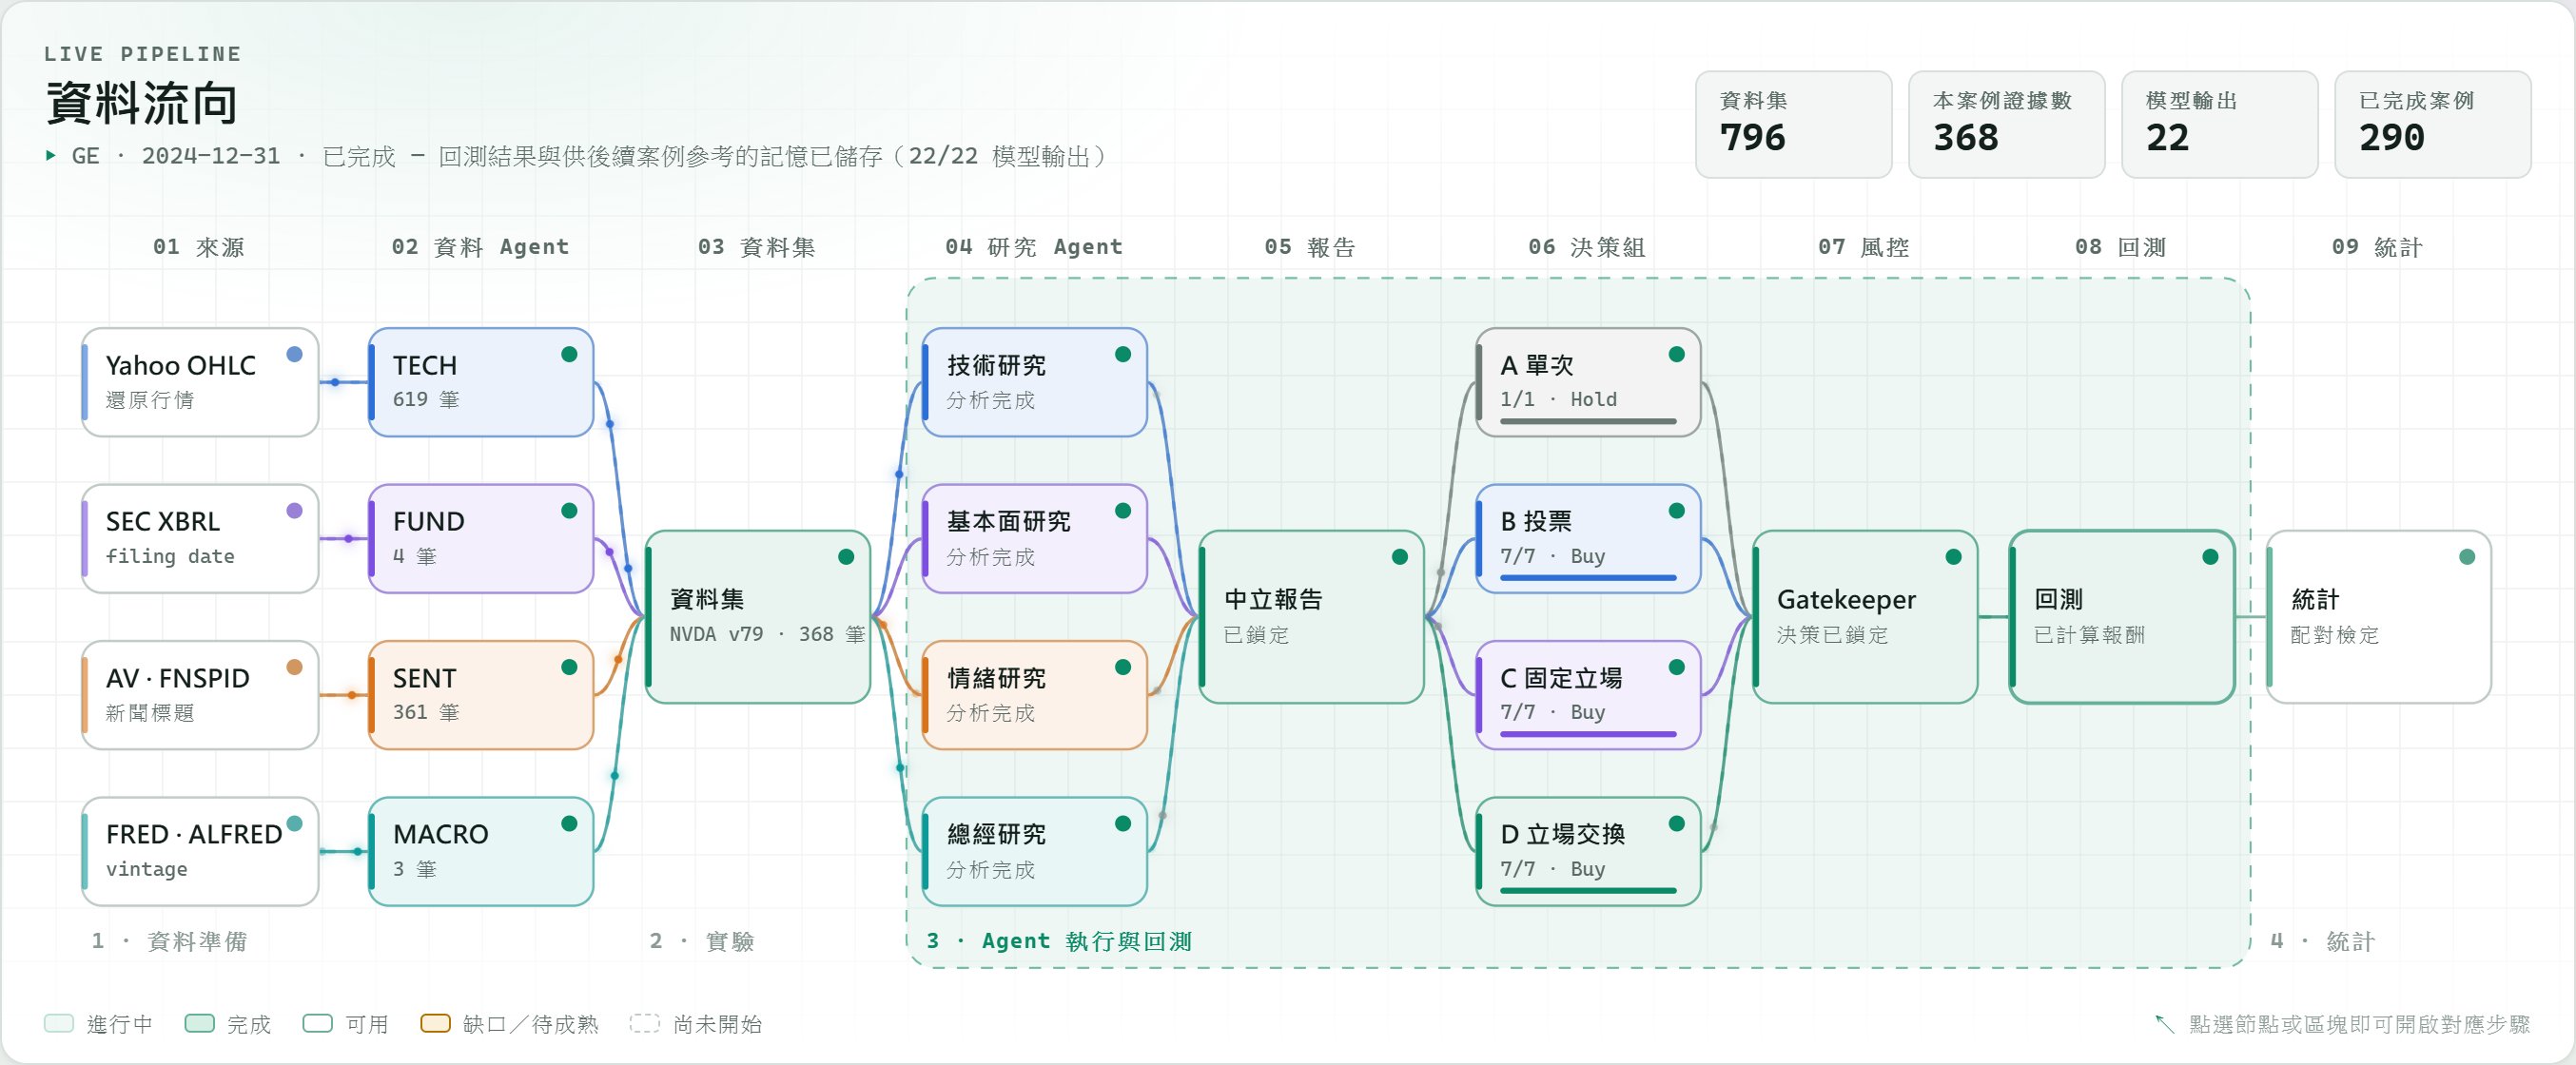
\includegraphics[width=\textwidth]{figures/ui-pipeline.png}
\caption{網頁介面之資料流向圖（一個已完成案例）。由左至右為資料來源、資料代理人、資料快照、研究代理人、中立報告、四組決策、守門員、回測與統計。}
\label{fig:ui}
\end{figure}

\subsection{四組決策機制}

四組使用相同的模型呼叫次數（表~\ref{tab:arms}），以排除「呼叫較多因而表現較佳」之解釋。每次決策輸出買進（做多）、持有（不進場）或賣出（放空），以及 60 個交易日之預期報酬、信心度、理由、引用證據與風險。

\begin{table}[H]
\centering\small
\caption{四組決策機制}
\label{tab:arms}
\begin{tabularx}{\textwidth}{@{}c l c Y@{}}
\toprule
組別 & 名稱 & 呼叫次數 & 流程 \\
\midrule
\grp{A} & 單次判斷 & 1 & 讀取報告後直接決策 \\
\grp{B} & 獨立投票 & 7 & 同一提示獨立取樣七次，多數決 \\
\grp{C} & 固定立場辯論 & 7 & 看多與看空辯論三輪（每輪可見雙方論述），再由裁決者決策 \\
\grp{D} & 立場交換辯論 & 7 & 第二輪交換立場、只見自己第一輪並須反駁之，第三輪換回，再由裁決者決策 \\
\bottomrule
\end{tabularx}
\end{table}

\subsection{立場交換辯論流程}

表~\ref{tab:rounds} 為立場交換組之三輪流程。第二輪隔離對手論述是刻意設計：若同時看得到對手，代理人容易轉為回應對手，而非檢討自己的主張；系統並核對代理人引用之「原主張」確實出自其第一輪文字。辯論組之裁決者須逐項核對雙方引用之證據，並綜合雙方論點在買進與賣出之間擇一。

\begin{table}[H]
\centering\small
\caption{立場交換辯論之三輪流程}
\label{tab:rounds}
\begin{tabularx}{\textwidth}{@{}l Y Y@{}}
\toprule
輪次 & 內容 & 目的 \\
\midrule
第 1 輪 & 看多與看空代理人各自提出論點並引用證據 & 建立正反兩方初始立場 \\
第 2 輪 & 雙方交換立場，只能看到自己第一輪之論述，須引用並反駁自己的原主張 & 迫使代理人檢驗自身論點之弱點 \\
第 3 輪 & 雙方換回原立場，整合前兩輪之論點與反駁 & 產生整合後之論點與不確定性揭露 \\
裁決 & 讀取完整辯論與報告，逐項核對證據後擇一方向 & 避免以辯論聲量決定 \\
\bottomrule
\end{tabularx}
\end{table}

\subsection{驗證與可稽核性}

為使每個決策可追溯，系統對模型輸出逐一驗證並留下紀錄：證據以短代稱（E1、E2、…）提供給模型，引用不存在之證據即要求重試；模型以證據代稱指稱事實而不重述數值，敘述中與來源不符之數字另行記錄；每個案例可匯出完整紀錄，包含資料快照、研究報告、辯論逐字稿、決策與回測結果。

%% =====================================================================
\section{實驗設計}
\label{sec:design}
%% =====================================================================

\subsection{資料與樣本}

樣本為九檔美國大型股（AAPL、\allowbreak NVDA、\allowbreak GOOGL、\allowbreak MSFT、\allowbreak AMZN、\allowbreak JPM、\allowbreak MCD、\allowbreak INTC、\allowbreak GE），分析日為 2021 至 2025 年共 20 個季末，合計 180 個案例。每個案例僅使用分析日前已公開之資料（表~\ref{tab:data}）。

\begin{table}[H]
\centering\small
\caption{資料來源與時間邊界}
\label{tab:data}
\begin{tabularx}{\textwidth}{@{}l l Y@{}}
\toprule
面向 & 來源 & 內容與時間處理 \\
\midrule
技術面 & 調整後日行情 & 近 20 日報酬、均線相對位置、年化波動度；僅用分析日前價格 \\
基本面 & SEC 財報 & 營收、淨利、營業現金流與去年同期比較；依申報日篩選 \\
情緒面 & 金融新聞標題（FNSPID、Alpha Vantage） & 分析日前 90 天全部標題，共 83,093 則，以 FinBERT 評分後彙整 \\
總經面 & FRED／ALFRED & 使用歷史版本，僅採分析日當時已發布之數值 \\
\bottomrule
\end{tabularx}
\end{table}

\subsection{偏誤控制}

\begin{itemize}
  \item \textbf{前視偏差}：資料依「可取得時間」而非事件時間篩選；股票代號與公司名稱於模型輸入中匿名化，降低模型憑記憶辨識標的的可能。
  \item \textbf{呼叫次數}：\grp{B}、\grp{C}、\grp{D} 皆為 7 次呼叫，讀取同一份研究報告。
  \item \textbf{事前登記}：180 個案例與分析計畫於執行前登記；程式與模型權重之版本於登記時鎖定，若有變動系統即拒絕執行，確保全部案例在同一規則下產生。
  \item \textbf{事前指定之主要檢定}：避免事後挑選有利的期間、成本或方法。
\end{itemize}

\subsection{評估方法}

於分析日後第一個交易日開盤進場、持有 60 個交易日後開盤出場，並扣除 Corwin--Schultz 估計之買賣價差成本 \citep{corwin2012spread}。主要比較事前指定為 \grp{D} 對 \grp{C}，兩個共同主要指標為方向準確率（配對 McNemar 檢定 \citep{mcnemar1947}）與年化 Sharpe 比率差（Ledoit--Wolf 檢定 \citep{ledoit2008sharpe}），並以 Holm 法 \citep{holm1979} 校正；兩者皆顯著為正才判定 \grp{D} 較佳。30 與 90 日、不計成本、排除低新聞量案例與以日期為群聚之信賴區間為敏感性分析。實驗模型為開源模型 qwen3:32b。

%% =====================================================================
\section{實驗結果}
\label{sec:results}
%% =====================================================================

\subsection{主要結果}

180 個事前登記案例全數完成，無排除案例。表~\ref{tab:main} 為四組之績效，表~\ref{tab:tests} 為配對檢定。

\begin{table}[H]
\centering\small
\caption{四組績效（180 案，60 個交易日，扣除交易成本）}
\label{tab:main}
\begin{tabular}{@{}lccccc@{}}
\toprule
組別 & 出手率 & 方向準確率 & 總報酬 & 最大回撤 & 年化 Sharpe \\
\midrule
\grp{A}\ 單次判斷 & 78.3\% & 56.0\% & 1.85\% & $-1.81\%$ & 0.44 \\
\grp{B}\ 獨立投票 & 79.4\% & 55.9\% & 1.95\% & $-1.83\%$ & 0.46 \\
\grp{C}\ 固定立場辯論 & 100\% & 58.3\% & 2.51\% & $-1.47\%$ & 0.59 \\
\grp{D}\ 立場交換辯論 & 100\% & 55.0\% & 2.11\% & $-2.01\%$ & 0.54 \\
\midrule
買進持有（相同期間） & -- & -- & 5.60\% & $-1.59\%$ & 1.01 \\
\bottomrule
\end{tabular}
\par\smallskip
\raggedright\footnotesize 出手率為買進或賣出（非持有）之比例；方向準確率以有出手之案例計算。報酬為 180 個案例等權重之組合結果。
\end{table}

\begin{table}[H]
\centering\small
\caption{立場交換組（\grp{D}）之配對檢定（60 個交易日）}
\label{tab:tests}
\begin{tabular}{@{}lcccccc@{}}
\toprule
比較 & 配對案例 & 方向不同 & 準確率差 & McNemar $p$ & Sharpe 差 & Ledoit--Wolf $p$ \\
\midrule
\grp{D} 對 \grp{C}（主要） & 180 & 16 & $-3.3$ & 0.21 & $-0.05$ & 0.80 \\
\grp{D} 對 \grp{B} & 143 & 9 & $+0.7$ & 1.00 & $+0.08$ & 0.79 \\
\grp{D} 對 \grp{A} & 141 & 8 & $+1.4$ & 0.73 & $+0.10$ & 0.72 \\
\bottomrule
\end{tabular}
\par\smallskip
\raggedright\footnotesize 準確率差單位為百分點。主要比較經 Holm 校正後之 $p$ 值為 0.42（準確率）與 0.80（Sharpe）。與 \grp{A}、\grp{B} 之比較以兩組皆出手之案例計算。
\end{table}

主要比較中，\grp{D} 之方向準確率與 Sharpe 比率皆略低於 \grp{C}，但差異不顯著。敏感性分析結果一致：以日期為群聚之準確率差 95\% 信賴區間為 $[-7.2, +0.6]$ 個百分點；30 與 90 日、不計成本、排除 37 個低新聞量案例後，差異方向相同且皆不顯著。四組皆未勝過同期買進持有。

\subsection{決策分布}

180 案中有 129 案（72\%）四組決策完全相同，\grp{C} 與 \grp{D} 僅 16 案方向不同。四組皆以買進為主（\grp{A} 108、\grp{B} 109、\grp{C} 145、\grp{D} 137 案）；\grp{D} 之賣出（42 案）多於 \grp{C}（34 案）。\grp{A} 與 \grp{B} 之決策幾乎相同，顯示七次投票之多數決大多與單次判斷一致。辯論兩組之 Sharpe 雖高於 \grp{A}、\grp{B}，但兩組必須出手，在以上漲為主之期間較少持有，此差異不能歸因於辯論本身。

\subsection{案例分析：自我反駁如何改變裁決}

以下兩個案例中 \grp{C} 與 \grp{D} 之方向不同。兩案之研究報告與模型完全相同，差別僅在辯論流程。

\paragraph{案例一：INTC 2024-03-31（\grp{D} 正確）。} 研究報告顯示新聞情緒偏正面、近 20 日報酬為正，但營收、淨利與營業現金流皆較去年同期大幅衰退。表~\ref{tab:case} 為兩組之辯論與裁決摘要（代理人原文為英文，此為摘譯）。

\begin{table}[H]
\centering\small
\caption{案例一：INTC 2024-03-31 之辯論與裁決（60 日實際報酬 $-30.5\%$）}
\label{tab:case}
\begin{tabularx}{\textwidth}{@{}l l Y@{}}
\toprule
組別／輪次 & 立場與預測 & 論點摘要 \\
\midrule
\grp{C} 第 1--3 輪 & 看多 $+8\%$；看空 $-12\%$ & 看多方三輪幾乎重複「情緒正面與短期動能支持看多」；看空方亦重複財報衰退，雙方未回應對方核心證據 \\
\grp{C} 裁決 & 買進，$+5\%$ & 採納看多方之短期動能論點 \\
\midrule
\grp{D} 第 1 輪 & 看多 $+8\%$；看空 $-10\%$ & 與 \grp{C} 相同之兩種論點 \\
\grp{D} 第 2 輪 & 原看多者改看空，$-7\%$ & 引用並反駁自己的原主張：正面情緒與短期報酬「被營收、淨利與現金流之大幅衰退所抵銷」 \\
\grp{D} 裁決 & 賣出，$-7\%$ & 基本面惡化之重要性高於短期情緒 \\
\bottomrule
\end{tabularx}
\end{table}

交換輪迫使原看多之代理人正視自己先前輕描淡寫的基本面衰退，裁決者因此轉為賣出；60 日後股價下跌 30.5\%，\grp{C} 是四組中唯一判斷錯誤者。

\paragraph{案例二：AAPL 2023-03-31（\grp{D} 錯誤）。} 同樣的機制也可能帶來反效果。此案技術面強勁（近 20 日上漲 11.3\%）但營收與淨利年減；\grp{C} 採納技術動能判斷買進，\grp{D} 之交換輪則再次強調基本面衰退，裁決者判斷賣出。60 日後股價上漲 15.3\%，\grp{D} 錯誤。

\paragraph{整體模式。} 在 16 個方向不同的案例中，\grp{D} 有 12 案判斷賣出，整體正確 5 案、錯誤 11 案。自我反駁使代理人更認真檢視原先被淡化的反面證據（多為基本面衰退），裁決者因此更常看空；此機制在基本面領先股價時有效，但本研究期間以上漲為主，「基本面疲弱而股價續漲」的情形較多，整體上反而降低準確率。

%% =====================================================================
\section{討論與結論}
\label{sec:conclusion}
%% =====================================================================

\subsection{結論}

在事前登記之 180 個季度案例中，自我反駁式立場交換辯論未優於固定立場辯論，兩組亦未勝過同期買進持有，與「辯論效果常被高估」之文獻一致 \citep{smit2023mad,zhang2025stop}。本研究之貢獻不在於證明某方法勝出，而在於以呼叫次數對齊、事前登記與版本鎖定之設計，在金融情境中提供可信的檢驗，並指出立場交換確實改變了模型的推理與立場，但「更謹慎地看待反面證據」不等於「更準確」。先前以較早版本流程進行之前導研究亦得到相同結論。

\subsection{研究限制}

第一，研究範圍為九檔美國大型股與 2021 至 2025 年，且期間以上漲為主，結論未必適用於空頭市場或其他標的。第二，匿名化僅隱藏代號與公司名稱，財報數值與日期仍可見，無法完全排除模型憑記憶辨識標的。第三，立場交換組同時包含「換到相反立場」與「暫時看不到對手」兩項設計，本研究未區分兩者各自的貢獻。第四，辯論組裁決者必須出手，與可持有之 \grp{A}、\grp{B} 之比較混合了此一差異。

\subsection{未來研究}

後續將（一）以每月一次之分析日擴充至 540 個案例，檢驗結論在不同時間尺度下是否一致；（二）以不同模型重複相同實驗，檢驗結論是否依賴特定模型；（三）新增「只看自己歷史但不換立場」之消融組，區分立場互換與資訊隔離之效果；（四）檢驗自我反駁在空頭或高波動期間是否反而有利。

\vspace{0.8cm}
\noindent\small 本文僅供學術研究與教學使用，不構成任何投資建議。
\normalsize

\clearpage
\bibliographystyle{chicago}
\bibliography{references}

\end{CJK}
\end{document}
